% !TeX program = xelatex
% Build from the repository root with build.ps1.
\documentclass[12pt,a4paper]{article}
\RequirePackage{array}[=2024-06-01]
% !TeX root = ../2/main.tex
\usepackage[a4paper,margin=25mm,headheight=16pt]{geometry}
\usepackage{amsmath,amssymb}
\usepackage{graphicx}
\usepackage{booktabs}
\usepackage{tabularx}
\usepackage{siunitx}
\usepackage{tikz}
\usepackage{circuitikz}
\usepackage[unicode,hidelinks]{hyperref}
\usepackage{xepersian}
% Only the regular B Nazanin file is installed; synthesize bold explicitly.
\settextfont[Path=C:/Windows/Fonts/,AutoFakeBold=2,AutoFakeSlant=0.2]{B-NAZANIN.TTF}
% B Nazanin lacks U+066A (Arabic percent), required by xepersian's digit setup.
% Arial covers the complete required digit/punctuation set; Persian prose remains B Nazanin.
\setdigitfont[Path=C:/Windows/Fonts/,BoldFont=arialbd.ttf,ItalicFont=ariali.ttf,BoldItalicFont=arialbi.ttf]{arial.ttf}
\setmathdigitfont[Path=C:/Windows/Fonts/,BoldFont=arialbd.ttf,ItalicFont=ariali.ttf,BoldItalicFont=arialbi.ttf]{arial.ttf}
\setlatintextfont{TeX Gyre Termes}
% B Nazanin does not contain the default itemize bullet and dash glyphs.
\renewcommand{\labelitemi}{\(\bullet\)}
\renewcommand{\labelitemii}{\(\circ\)}
\renewcommand{\labelitemiii}{\(\diamond\)}
\setlength{\parindent}{0pt}
\setlength{\parskip}{0.5em}
\linespread{1.25}
\newcommand{\exercise}[1]{\section*{تمرین #1}}
% !TeX root = ../2/main.tex
% Shared title page for every assignment.
% Change only \AssignmentNumber and \AssignmentDate in each main document.

\newcommand{\AssignmentNumber}[1]{\gdef\assignmentnumber{#1}}
\newcommand{\AssignmentDate}[1]{\gdef\assignmentdate{#1}}

\newcommand{\assignmentnumber}{---}
\newcommand{\assignmentdate}{---}

% Stable course metadata
\newcommand{\universityname}{دانشگاه صنعتی امیرکبیر}
\newcommand{\universityalias}{پلی‌تکنیک تهران}
\newcommand{\facultyname}{دانشکده مهندسی کامپیوتر}
\newcommand{\coursename}{طراحی مدارهای مجتمع پرتراکم پیشرفته}
\newcommand{\studentname}{محمد خلیلی اصل}
\newcommand{\instructorname}{دکتر مهدی صدیقی}

\newcommand{\MakeAssignmentCover}{%
  \begin{titlepage}
    \thispagestyle{empty}
    \centering
    \linespread{1}\selectfont

    \vspace*{0mm}
    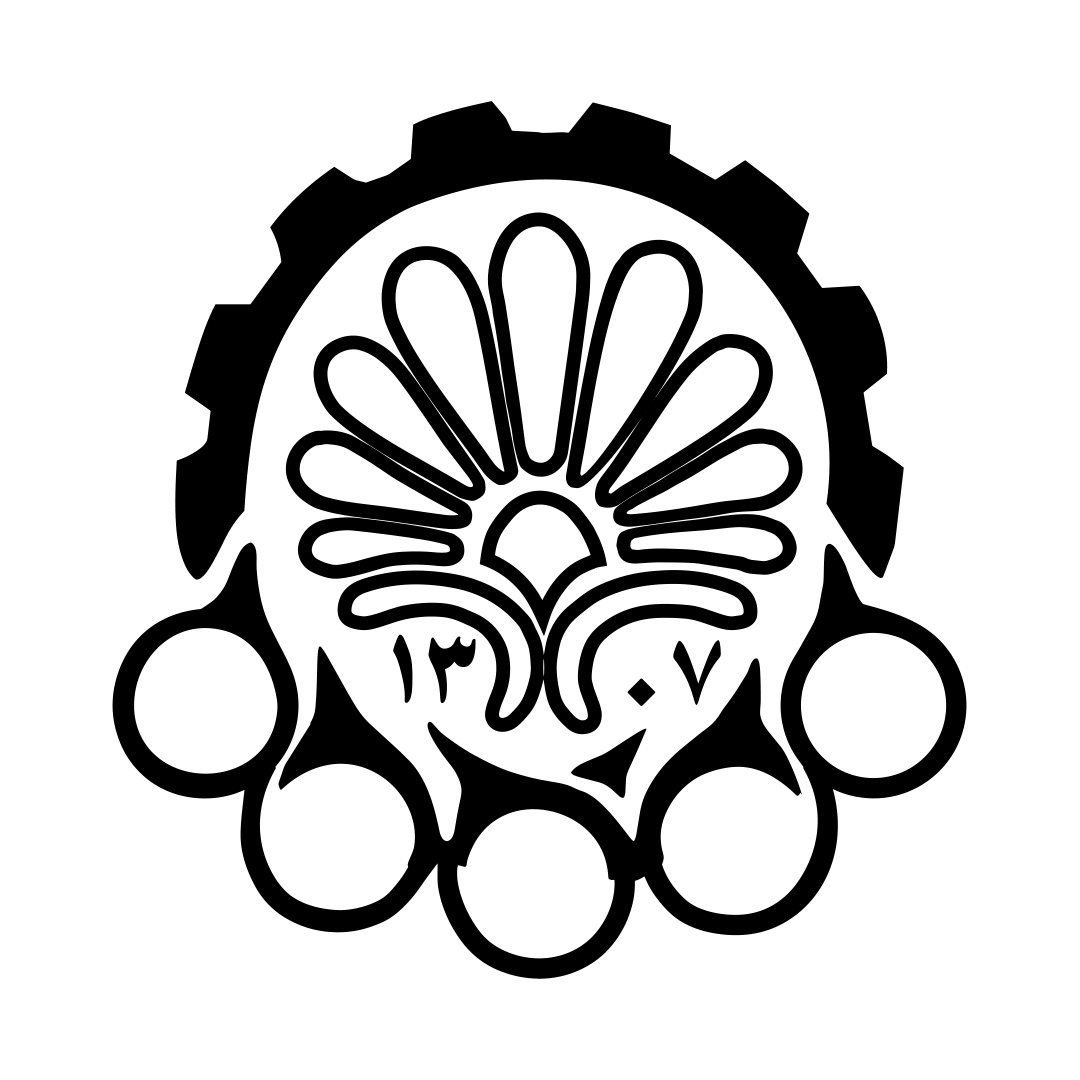
\includegraphics[width=44mm]{assets/aut-logo-black.png}\par
    \vspace{3mm}

    {\Large\bfseries \universityname\par}
    \vspace{1mm}
    {\large (\universityalias)\par}
    \vspace{1mm}
    {\large \facultyname\par}

    \vspace{8mm}
    {\Large\bfseries درس \coursename\par}

    \vspace{12mm}
    {\large عنوان\par}
    \vspace{2mm}
    {\LARGE\bfseries تمرین شماره \assignmentnumber\par}

    \vspace{10mm}
    {\large تهیه‌کننده\par}
    \vspace{2mm}
    {\Large\bfseries \studentname\par}

    \vspace{10mm}
    {\large استاد درس\par}
    \vspace{2mm}
    {\Large\bfseries \instructorname\par}

    \vspace{10mm}
    {\Large \assignmentdate\par}
    \vfill
  \end{titlepage}
  \setcounter{page}{1}%
}


\XeTeXgenerateactualtext=1
% Preserve logical order of dotted Persian section identifiers.
\newcommand{\secnum}[1]{\mbox{\beginL#1\endL}}
\setlength{\emergencystretch}{3em}
\hypersetup{pdftitle={جزوه اول؛ فهرست تفصیلی و نمونه آموزشی}}
% Reuse the canonical cover without changing its shared definition.
\AssignmentNumber{جزوه اول؛ فهرست و نمونه آموزشی}
\AssignmentDate{نسخه مقدماتی برای بررسی}
\patchcmd{\MakeAssignmentCover}{تمرین شماره \assignmentnumber}{\assignmentnumber}{}{\errmessage{Cover title replacement failed}}
\begin{document}
\MakeAssignmentCover
% !TeX root = booklet-01-preview.tex
\section*{هدف و روش مطالعه}
این جزوه برای دانشجویی تنظیم می‌شود که درس الکترونیک دیجیتال را نگذرانده است.
پیش‌نیازهای مدار، منطق و ریاضی در محل مناسب آموزش داده می‌شوند؛ بنابراین آشنایی قبلی
با تحلیل ترانزیستور، مشتق یا انتگرال فرض نمی‌شود. هدف، رسیدن از شناخت کمیت‌های مدار
به فهم روابط جریان و ظرفیت \lr{MOSFET} است.

\textbf{وضعیت این نسخه:} فقط فهرست تفصیلی پیشنهادی و یک نمونه آموزشی نوشته شده است.
عنوان‌های فهرست، به معنای تکمیل آن درس‌ها نیستند. نمونه، میزان توضیح و شیوه ارائه را
نشان می‌دهد؛ آموزش کامل پیش‌نیازها در نسخه نهایی گسترده‌تر خواهد بود.

دامنه جزوه اول، کل فصل ۱ و بخش‌های \secnum{۲.۱} تا \secnum{۲.۳} کتاب است \cite{weste}.
اسلایدهای \lr{00} و \lr{01} راهنمای ترتیب و تاکید درس‌اند \cite{intro,mos}؛
مطالب کتاب که در اسلایدها کوتاه شده‌اند نیز با ارجاع روشن پوشش داده می‌شوند.
مثال‌های تکمیلی با عنوان «مثال آموزشی» از مثال‌های کتاب متمایز خواهند بود.

\section*{فهرست تفصیلی پیشنهادی جزوه اول}
\subsection*{بخش آغازین: پیش‌نیازهای ضروری}
\begin{enumerate}
\item \textbf{کمیت‌ها و واحدها:} بار، جریان، ولتاژ، انرژی و توان؛ جهت مرجع؛
\lr{Ground} و اختلاف پتانسیل؛ واحدهای \lr{SI} و پیشوندها.
\item \textbf{ریاضی محاسبات مدار:} کسر و نسبت، توان و نماد علمی، تبدیل واحد،
جابه‌جایی جمله‌ها، پرانتز، معادله خطی و درجه‌دو؛ انتخاب جواب سازگار با مسئله.
\item \textbf{مدارهای پایه:} مقاومت و \lr{Ohm's Law}، مدار باز و اتصال کوتاه،
\lr{Node} و \lr{Branch}؛ اتصال \lr{Series} و \lr{Parallel}؛
\lr{Kirchhoff's Current Law (KCL)} و \lr{Kirchhoff's Voltage Law (KVL)}.
\item \textbf{خازن و زمان:} بار ذخیره‌شده، رابطه بار و ولتاژ، شارژ و دشارژ؛
تفاوت حالت ماندگار و گذرا؛ مقدمه نرخ تغییر و شیب با نمودار.
\item \textbf{منطق دیجیتال:} تفاوت \lr{Analog} و \lr{Digital}؛
سطح ولتاژ و مقدار منطقی؛ \lr{Truth Table} و گیت‌های
\lr{NOT, AND, OR, NAND, NOR, XOR, XNOR}.
\item \textbf{جبر و ساختار منطق:} \lr{Boolean Algebra} و \lr{De Morgan's Laws}؛
ساخت گیت از \lr{Switch}؛ تفاوت \lr{Combinational} و \lr{Sequential}؛
مفهوم حافظه و \lr{Clock}، با مثال ساده.
\end{enumerate}

\clearpage
\subsection*{فصل اول: از ترانزیستور تا فرایند طراحی}
ترتیب زیر تمام بخش‌های \secnum{۱.۱} تا \secnum{۱.۱۲} را پوشش می‌دهد؛ مرزها با فهرست کتاب تطبیق
داده شده‌اند \cite{weste}. هر درس شامل توضیح، مثال و پرسش با پاسخ خواهد بود.
\begin{enumerate}
\item \textbf{بخش‌های \secnum{۱.۱} و \secnum{۱.۲}:} تاریخچه \lr{IC} و \lr{VLSI}،
\lr{Moore's Law} و مسیر کلی طراحی؛ خواندن رشد نمایی و نمودار نیمه‌لگاریتمی.
آمار تاریخی منبع، با تاریخ خود آن گزارش می‌شود.
\item \textbf{بخش \secnum{۱.۳}:} ساختار ابتدایی \lr{MOS}، چهار پایانه،
کنترل مسیر جریان با ولتاژ \lr{Gate}، مقایسه \lr{nMOS} و \lr{pMOS} و مدل \lr{Switch}.
\item \textbf{بخش \secnum{۱.۴}:} طراحی \lr{Inverter}، \lr{NAND} و \lr{NOR}؛
شبکه‌های \lr{Pull-up} و \lr{Pull-down} و گیت‌های \lr{Compound}؛
\lr{Pass Transistor}، \lr{Transmission Gate}، \lr{Tristate}،
\lr{Multiplexer} و مدارهای \lr{Sequential}.
\item \textbf{بخش \secnum{۱.۵}:} مقطع \lr{Inverter}، مراحل \lr{Fabrication}،
\lr{Layout Design Rules}، \lr{Gate Layout} و \lr{Stick Diagram}؛
ارتباط نمای مداری و فیزیکی با شکل‌های خوانا.
\item \textbf{بخش \secnum{۱.۶}:} \lr{Design Partitioning}، \lr{Abstraction}،
\lr{Hierarchy}، \lr{Regularity} و \lr{Modularity}؛
دامنه‌های \lr{Behavioral}، \lr{Structural} و \lr{Physical}.
\item \textbf{بخش \secnum{۱.۷}:} معرفی مقدمات لازم برای مثال \lr{MIPS}،
تفاوت \lr{Architecture} و \lr{Microarchitecture} و اجرای چندچرخه‌ای؛
ساختار پردازنده پیش از تحلیل مثال کتاب معرفی می‌شود.
\item \textbf{بخش \secnum{۱.۸}:} \lr{Logic Design}، رابط‌های سطح بالا، نمودار بلوکی،
سلسله‌مراتب و \lr{Hardware Description Language (HDL)}؛
خواندن مثال‌های کتاب بدون فرض آشنایی قبلی با کدنویسی سخت‌افزار.
\item \textbf{بخش \secnum{۱.۹}:} \lr{Circuit Design}؛ مقدمه معیارهای
\lr{Delay}، \lr{Power} و \lr{Area} در حد همین فصل و پیوند آن‌ها با ترانزیستور.
\item \textbf{بخش \secnum{۱.۱۰}:} \lr{Floorplanning}، \lr{Standard Cell}،
\lr{Pitch Matching}، \lr{Slice Plan}، \lr{Array} و برآورد مساحت.
\item \textbf{بخش‌های \secnum{۱.۱۱} و \secnum{۱.۱۲}:} هدف و سطوح \lr{Verification}؛
\lr{Fabrication}، \lr{Packaging} و \lr{Testing} و تفاوت نقش آن‌ها.
\end{enumerate}

\clearpage
\subsection*{ابتدای فصل دوم: از ساختار فیزیکی تا مدل ریاضی}
\begin{enumerate}
\item \textbf{بخش \secnum{۲.۱}:} ساختار \lr{Silicon}، \lr{Doping}،
\lr{Electron} و \lr{Hole}، پیوند \lr{PN} و بایاس آن؛
ساختار \lr{MOS} و حالت‌های \lr{Accumulation}، \lr{Depletion} و \lr{Inversion}؛
تعریف \lr{Threshold Voltage} و ولتاژهای پایانه‌ها.
\item \textbf{بخش \secnum{۲.۲}، مقدمات:} نقش \(W\)، \(L\)، \(t_{\mathrm{ox}}\)،
\(\mu\) و \(C_{\mathrm{ox}}\)؛ تفاوت ظرفیت و ظرفیت بر واحد سطح؛
میدان الکتریکی و سرعت حامل، با کنترل واحدها.
\item \textbf{بخش \secnum{۲.۲}، استخراج:} بار کانال، جریان \lr{Long-Channel} و
مفهوم انتگرال به‌عنوان جمع سهم‌های کوچک؛ استخراج روابط \lr{Linear} و
\lr{Saturation} و پیوستگی مرز؛ قرارداد علامت‌ها در \lr{pMOS}؛
حل مثال با تعیین ناحیه پیش و پس از محاسبه.
\item \textbf{بخش \secnum{۲.۳.۱}:} مدل ساده \lr{Gate Capacitance} و
\lr{Diffusion Capacitance}؛ اثر هندسه و اشتراک ناحیه‌های \lr{Diffusion}.
\item \textbf{بخش \secnum{۲.۳.۲}:} مدل تفصیلی ظرفیت \lr{Gate}، سهم پایانه‌ها،
\lr{Overlap} و وابستگی ظرفیت‌ها به ناحیه عملکرد.
\item \textbf{بخش \secnum{۲.۳.۳}:} مدل تفصیلی ظرفیت پیوند، سهم مساحت و محیط جانبی،
وابستگی به بایاس و مفهوم ظرفیت موثر در تغییر ولتاژ.
\end{enumerate}

\subsection*{جمع‌بندی و پیوند با دو جزوه بعدی}
در پایان جزوه، جدول نمادها و واحدها، نقشه انتخاب مدل، فرمول‌ها همراه با شرط اعتبار،
خطاهای رایج و پرسش‌های ترکیبی با پاسخ تشریحی قرار می‌گیرند.
بخش \secnum{۲.۴} به جزوه دوم و بخش \secnum{۲.۵} به جزوه سوم تعلق دارد؛ در جزوه اول فقط
ضرورت آن‌ها معرفی می‌شود. مشتق‌گیری تفصیلی برای \lr{Noise Margin} در جزوه سوم
آموزش داده خواهد شد.

\textbf{معیار پوشش:} برای هر عنوان کتاب در دامنه تعیین‌شده، توضیح آموزشی و ارجاع
قابل‌ردیابی ارائه می‌شود. منظور، بازنویسی آموزشی مفاهیم و استدلال‌هاست؛
متن کتاب یا تمام تمرین‌های پایان فصل عیناً بازتولید نمی‌شوند.

\clearpage
% !TeX root = booklet-01-preview.tex
\section{نمونه آموزشی: ولتاژ و جریان}
\label{sec:electrical-basics}
هدف این نمونه آن است که بتوانیم عملکرد یک \lr{CMOS Inverter} را از روی
اتصال‌های مدار توضیح دهیم. ابتدا کمیت‌های لازم را می‌شناسیم و سپس از یک مدل ساده
برای ترانزیستور استفاده می‌کنیم. بخش مقدماتی این نمونه، توضیح تکمیلی برای ورود
به مدل \lr{Switch} در بخش \secnum{۱.۳} کتاب است؛ مثال‌های عددی آن، داده فناوری یا نتیجه شبیه‌سازی نیستند.

\subsection{بار و جریان چه تفاوتی دارند؟}
بار الکتریکی را با \(Q\) و واحد \lr{coulomb} با نماد \(\mathrm{C}\) نمایش می‌دهیم.
جریان، آهنگ عبور بار از یک مقطع است. اگر در مدت \(\Delta t\)، بار خالص
\(\Delta Q\) در جهت مرجع از مقطع عبور کند، جریان متوسط برابر است با:
\begin{equation}\label{eq:average-current}
I_{\mathrm{avg}}=\frac{\Delta Q}{\Delta t}.
\end{equation}
علامت \(\Delta\) یعنی «تغییر» یا «اختلاف»؛ در اینجا \(\Delta t\) طول بازه زمانی است.
کسر در رابطه \eqref{eq:average-current} یعنی مقدار بار را بر مدت عبور آن تقسیم می‌کنیم.
واحد جریان \lr{ampere} است و \(\qty{1}{\ampere}=\qty{1}{\coulomb\per\second}\).
جهت جریان قراردادی، جهت حرکت بار مثبت است؛ حرکت \lr{Electron} در فلز در جهت مخالف آن است.

\textbf{مثال آموزشی.} فرض کنید در مدت \(\qty{2}{\nano\second}\)، بار خالص
\(\qty{6}{\pico\coulomb}\) در جهت مرجع از یک مقطع عبور کند.
پیشوندهای \lr{pico} و \lr{nano} به‌ترتیب به معنی \(10^{-12}\) و \(10^{-9}\) هستند.
جای‌گذاری، همراه با تبدیل واحد، می‌دهد:
\begin{align}
I_{\mathrm{avg}}
&=\frac{6\times10^{-12}\,\mathrm{C}}{2\times10^{-9}\,\mathrm{s}}
=\frac{6}{2}\times10^{-12-(-9)}\,\mathrm{A}\notag\\
&=3\times10^{-3}\,\mathrm{A}=\qty{3}{\milli\ampere}.
\end{align}
در تقسیم توان‌های هم‌پایه، توان مخرج از توان صورت کم می‌شود؛ بنابراین
\(-12-(-9)=-3\). این نتیجه جریان متوسط است؛ از آن نمی‌توان ثابت‌بودن جریان
در تمام لحظه‌های بازه را نتیجه گرفت.

\subsection{ولتاژ همیشه نسبت به یک مرجع است}
ولتاژ، اختلاف پتانسیل الکتریکی است؛ از دید انرژی، اختلاف پتانسیل دو نقطه نشان می‌دهد
به‌ازای هر واحد بار مثبت، انرژی پتانسیل چقدر تفاوت دارد.
واحد آن \lr{volt} است: \(\qty{1}{\volt}=\qty{1}{\joule\per\coulomb}\).
اگر پتانسیل دو نقطه \(a\) و \(b\) نسبت به یک مرجع، \(V_a\) و \(V_b\) باشد، تعریف می‌کنیم:
\begin{equation}\label{eq:voltage-difference}
V_{ab}=V_a-V_b.
\end{equation}
پس اگر \(V_a=\qty{1}{\volt}\) و \(V_b=\qty{0.4}{\volt}\)،
داریم \(V_{ab}=\qty{0.6}{\volt}\)، ولی \(V_{ba}=\qty{-0.6}{\volt}\).
عوض‌کردن ترتیب پایانه‌ها علامت را تغییر می‌دهد؛ این نکته در تعریف \(V_{gs}\) مهم خواهد بود.

\clearpage
\subsection{مرجع، اتصال و شرط عبور جریان}
\lr{Ground} گره‌ای است که پتانسیل آن را در تحلیل صفر در نظر می‌گیریم.
هر \lr{Node}، مجموعه نقاط متصل با سیم ایدئال است که پتانسیل یکسان دارند.
\lr{Ground} لزوماً اتصال فیزیکی به زمین نیست؛ صفر بودن ولتاژ یک گره نیز
به معنی نبود بار یا نبود جریان در تمام شاخه‌های متصل به آن نیست.

وجود ولتاژ به‌تنهایی برای عبور جریان از هر مسیر دلخواه کافی نیست؛ مسیر باید امکان
هدایت داشته باشد. در مدل ایدئال، \lr{Open Circuit} مسیر هدایت را قطع می‌کند،
درحالی‌که \lr{Short Circuit} اختلاف ولتاژ دو سر خود را صفر می‌کند.
جریان اتصال کوتاه را سایر اجزای مدار تعیین می‌کنند؛ نمی‌توان گفت همیشه صفر یا همیشه بی‌نهایت است.

برای یک مقاومت مثبت \(R\)، جریان مرجع \(I\) را از سر با علامت مثبت ولتاژ \(V\)
به سر منفی انتخاب می‌کنیم. در مدل مقاومت خطی، \lr{Ohm's Law} می‌گوید:
\begin{equation}\label{eq:ohm}
V=RI\quad\Longrightarrow\quad I=\frac{V}{R}.
\end{equation}
برای رسیدن به عبارت دوم، دو طرف عبارت اول را بر \(R\) تقسیم کرده‌ایم.
واحد مقاومت \lr{ohm} است. اگر \(V=\qty{1}{\volt}\) و
\(R=\qty{1}{\kilo\ohm}=\qty{1000}{\ohm}\)، جریان
\(I=\qty{0.001}{\ampere}=\qty{1}{\milli\ampere}\) خواهد بود.
این قانون مدل مقاومت است؛ هنوز مجاز نیستیم آن را مدل دقیق ترانزیستور بدانیم.

\section{از ولتاژ به صفر و یک منطقی}
مقدار منطقی با مقدار ولتاژ یکسان نیست. برای نمونه، در مدار آموزشی با تغذیه
\(V_{\mathrm{DD}}=\qty{1}{\volt}\)، ولتاژ نزدیک صفر را نماینده صفر منطقی و
ولتاژ نزدیک تغذیه را نماینده یک منطقی می‌گیریم.
عدد یک منطقی واحد ندارد؛ \(\qty{1}{\volt}\) یک کمیت فیزیکی است.
تغذیه انتخاب‌شده فقط برای مثال است و مشخصات فناوری خاصی را بیان نمی‌کند.

در مدار واقعی، صفر و یک با بازه‌های مجاز ولتاژ تعریف می‌شوند؛ هر ولتاژ میانی
الزاماً یک مقدار منطقی معتبر نیست. در این نمونه فقط دو ورودی دقیقاً برابر
صفر و \(V_{\mathrm{DD}}\) را تحلیل می‌کنیم. تحلیل بازه‌ها و تحمل نویز در جزوه سوم می‌آید.
این شیوه نمایش سطوح با معرفی کتاب سازگار است \cite[بخش \secnum{۱.۳}، صفحه چاپی ۸]{weste}.

\textbf{نکته کلیدی.} صفر بودن ورودی یعنی ولتاژ آن نسبت به \lr{Ground} صفر است؛
این عبارت به معنی قطع‌بودن همه ترانزیستورهای مدار نیست. نوع ترانزیستور و اختلاف
ولتاژ پایانه‌های آن تعیین می‌کنند کدام مسیر هدایت دارد.

\clearpage
\section{ترانزیستور به‌عنوان \lr{Switch}}
\subsection{پایانه کنترل را از مسیر هدایت جدا کنیم}
ترانزیستور \lr{MOSFET} چهار پایانه \lr{Gate}، \lr{Source}، \lr{Drain} و
\lr{Body} دارد. در مدل مقدماتی، ولتاژ \lr{Gate} وضعیت مسیر میان
\lr{Source} و \lr{Drain} را کنترل می‌کند. جریان مسیر هدایت از خود
\lr{Gate} عبور نمی‌کند؛ در مدل ایدئال، عایق \lr{Gate} جریان رسانشی آن را صفر می‌کند.
بااین‌حال، برای تغییر ولتاژ \lr{Gate} باید ظرفیت آن شارژ یا دشارژ شود؛
پس این مدل، نبود هر نوع جریان ورودی در هنگام تغییر را ثابت نمی‌کند
\cite[بخش \secnum{۱.۳}]{weste}\cite[اسلایدهای ۵ تا ۸]{mos}.

ولتاژ کنترل \lr{nMOS} را \(V_{gs}=V_g-V_s\) می‌نامیم؛ بنابراین
فقط دانستن \(V_g\) کافی نیست. در \lr{Inverter} این نمونه،
\lr{Source} ترانزیستور \lr{nMOS} به صفر و \lr{Source} ترانزیستور \lr{pMOS}
به \(V_{\mathrm{DD}}\) متصل است. بدنه‌ها نیز به‌ترتیب به همین ریل‌ها متصل‌اند.
فرض می‌کنیم تغذیه برای روشن‌شدن هر ترانزیستور در ورودی مناسب کافی است.

\subsection{قاعده کنترل در همین اتصال مشخص}
با اتصال‌های یادشده، ورودی بالا \lr{nMOS} را روشن و \lr{pMOS} را خاموش می‌کند؛
ورودی پایین نتیجه معکوس دارد. این همان مدل \lr{Switch} کتاب و اسلاید است
\cite[صفحه چاپی ۸]{weste}\cite[اسلاید ۲۱]{intro}.
در این مدل، \lr{ON} یعنی مسیر بسته و \lr{OFF} یعنی مسیر باز.
\textbf{روشن بودن، وجود مسیر را بیان می‌کند؛ جریان غیرصفر را تضمین نمی‌کند.}
اگر اختلاف ولتاژ لازم وجود نداشته باشد، مسیر روشن نیز می‌تواند جریان صفر داشته باشد.

جدول \ref{tab:switch} فقط برای دو ورودی ریل‌به‌ریل و اتصال‌های همین نمونه است؛
قاعده عمومی برای همه مدارهای \lr{Pass Transistor} نیست.
\begin{table}[ht]
\centering
\caption{وضعیت مدل \lr{Switch} در اتصال مخصوص \lr{Inverter}}
\label{tab:switch}
\begin{tabular}{ccc}
\toprule
ورودی & \lr{nMOS} & \lr{pMOS}\\
\midrule
صفر منطقی & قطع & وصل\\
یک منطقی & وصل & قطع\\
\bottomrule
\end{tabular}
\end{table}

\textbf{حد اعتبار.} مقاومت مسیر روشن، \lr{Leakage} و روند زمانی تغییر وضعیت
در این مدل حذف شده‌اند. روابط جریان و ناحیه‌های عملکرد در ادامه جزوه اول،
و اثرهای \lr{Nonideal} در جزوه دوم آموزش داده خواهند شد.

\clearpage
\section{ساخت و تحلیل \lr{CMOS Inverter}}
\subsection{ابتدا اتصال‌ها را بخوانیم}
\lr{Complementary Metal-Oxide-Semiconductor (CMOS)} از دو نوع مکمل
ترانزیستور استفاده می‌کند. در \lr{Inverter} شکل \ref{fig:inverter}،
\lr{Gate} هر دو ترانزیستور ورودی مشترک \(A\) دارد و اتصال مشترک
\lr{Drain}ها خروجی \(Y\) است. ترانزیستور بالایی مسیر \lr{Pull-up}
از تغذیه به خروجی و ترانزیستور پایینی مسیر \lr{Pull-down} از خروجی به زمین را می‌سازد
\cite[بخش \secnum{۱.۴.۱}، صفحه چاپی ۹]{weste}.

\begin{figure}[ht]
\centering
\begin{latin}
\begin{circuitikz}[american,scale=1.05]
\draw (0,3) node[pmos] (p) {};
\draw (0,0) node[nmos] (n) {};
\draw (p.S) -- (0,4.2) node[above] {$V_{\mathrm{DD}}$};
\draw (n.S) -- (0,-1.2) node[ground] {};
\draw (p.D) -- (0,1.5) -- (n.D);
\draw (0,1.5) to[short,*-o] (2,1.5) node[right] {$Y$};
\draw (p.G) -- (-1.7,3) -- (-1.7,0) -- (n.G);
\draw (-1.7,1.5) to[short,*-o] (-2.6,1.5) node[left] {$A$};
\node[right] at (0.6,3) {pMOS};
\node[right] at (0.6,0) {nMOS};
\end{circuitikz}
\end{latin}
\caption{بازترسیم آموزشی \lr{CMOS Inverter} بر پایه شکل \secnum{۱.۱۱} کتاب و اسلاید ۲۳
\cite{weste,intro}. بدنه‌ها در نماد ساده نمایش داده نشده‌اند؛ اتصال آن‌ها در متن مشخص است.}
\label{fig:inverter}
\end{figure}

سیم ورودی به \lr{Gate}ها می‌رود و از مسیر خروجی جداست.
در سمت چپ شکل، نقطه اتصال نشان می‌دهد هر دو \lr{Gate} ولتاژ یکسان می‌گیرند.
حباب کوچک کنار \lr{Gate} ترانزیستور بالا نشانه \lr{pMOS} است.
خط‌های اتصال، سیم ایدئال‌اند؛ از روی شکل نباید مسیر رسانشی مستقیمی از \(A\) به \(Y\) فرض کرد.

\clearpage
\subsection{ورودی صفر: چرا خروجی یک می‌شود؟}
فرض می‌کنیم \(V_A=\qty{0}{\volt}\).
\lr{nMOS} خاموش است، زیرا \(V_{gs,n}=V_A-0=0\).
\lr{pMOS} روشن است، زیرا اختلاف ولتاژ کنترل مناسب آن
\(V_{sg,p}=V_{\mathrm{DD}}-V_A=V_{\mathrm{DD}}\) است.
پس مسیر خروجی به زمین قطع و مسیر آن به تغذیه وصل می‌شود.
در حالت ماندگار مدل ایدئال و بدون بار رسانشی خروجی، نتیجه می‌گیریم:
\begin{equation}\label{eq:inverter-low}
V_A=0\quad\Longrightarrow\quad V_Y=V_{\mathrm{DD}}.
\end{equation}
اگر خروجی ابتدا ولتاژ کمتری داشته باشد، ظرفیت آن از مسیر بالایی شارژ می‌شود؛
نتیجه \eqref{eq:inverter-low} مقدار نهایی است و زمان رسیدن به آن را تعیین نمی‌کند.

\subsection{ورودی یک: چرا خروجی صفر می‌شود؟}
اکنون \(V_A=V_{\mathrm{DD}}\). برای \lr{pMOS} داریم
\(V_{sg,p}=V_{\mathrm{DD}}-V_A=0\)، پس خاموش است.
برای \lr{nMOS} داریم \(V_{gs,n}=V_{\mathrm{DD}}\)، پس روشن است.
خروجی از تغذیه جدا و به زمین متصل می‌شود. در همان مدل و حالت ماندگار:
\begin{equation}\label{eq:inverter-high}
V_A=V_{\mathrm{DD}}\quad\Longrightarrow\quad V_Y=0.
\end{equation}
اگر ظرفیت خروجی قبلاً شارژ شده باشد، از مسیر پایینی دشارژ می‌شود.
جدول \ref{tab:inverter} دو نتیجه را به زبان منطق بیان می‌کند.

\begin{table}[ht]
\centering
\caption{جدول درستی \lr{Inverter} در مدل ایدئال و حالت ماندگار}
\label{tab:inverter}
\begin{tabular}{cc}
\toprule
ورودی \(A\) & خروجی \(Y\)\\
\midrule
۰ & ۱\\
۱ & ۰\\
\bottomrule
\end{tabular}
\end{table}

عملکرد منطقی با \(Y=\overline{A}\) نمایش داده می‌شود؛ خط بالای \(A\)
علامت \lr{NOT} است و به معنی منفی عددی نیست. این جدول را از اتصال‌ها استخراج کردیم؛
صرفاً نام گیت را حفظ نکردیم.

\clearpage
\section{کنترل فهم و مرز نتیجه}
در هر دو حالت پایدار بررسی‌شده، یکی از دو ترانزیستور قطع است؛ بنابراین
در مدل ایدئال مسیر رسانشی پیوسته‌ای از تغذیه به زمین نداریم.
این نتیجه به معنی صفر بودن توان واقعی مدار در همه شرایط نیست:
هنگام تغییر ورودی، ظرفیت‌ها شارژ و دشارژ می‌شوند، ممکن است دو ترانزیستور
برای مدتی هم‌زمان هدایت کنند و در مدار واقعی \lr{Leakage} نیز وجود دارد.
این محدودیت‌ها مانع استفاده آموزشی از مدل ساده نمی‌شوند؛ محدوده نتیجه را مشخص می‌کنند.

\subsection{پرسش‌ها و پاسخ‌های تشریحی}
\begin{enumerate}
\item \textbf{اگر ورودی صفر باشد، چرا خروجی هم صفر نیست؟}
ورودی به \lr{Gate}ها وصل است، نه مستقیماً به خروجی.
صفر شدن ورودی، ترانزیستور بالا را روشن می‌کند و خروجی به تغذیه می‌رسد.
\item \textbf{آیا ترانزیستور روشن همیشه جریان می‌دهد؟}
خیر. روشن بودن امکان هدایت را فراهم می‌کند. پس از رسیدن خروجی بی‌بار
به ریل مربوط، جریان ماندگار مدل ایدئال می‌تواند صفر شود.
\item \textbf{چرا در تعریف ولتاژ کنترل، ولتاژ \lr{Source} را کم می‌کنیم؟}
کنترل با اختلاف پتانسیل انجام می‌شود، نه با ولتاژ مطلق \lr{Gate}.
برای مثال، اگر \(V_g=\qty{1}{\volt}\) و \(V_s=\qty{0.4}{\volt}\)،
آنگاه \(V_{gs}=\qty{0.6}{\volt}\)، نه \(\qty{1}{\volt}\).
روشن بودن به مقایسه این اختلاف با آستانه نیاز دارد؛ مقدار آستانه در این مثال داده نشده است.
\item \textbf{اگر هر دو مسیر قطع شوند، آیا خروجی الزاماً صفر است؟}
خیر. خروجی می‌تواند \lr{Floating} باشد و بار قبلی را روی ظرفیت خود نگه دارد.
مدل ساده بدون شرایط اولیه، ولتاژ یکتایی تعیین نمی‌کند.
اگر هر دو مسیر روشن شوند نیز یک مسیر از تغذیه به زمین ایجاد می‌شود؛
برای محاسبه جریان و ولتاژ آن باید مدل دقیق‌تری داشت
\cite[صفحه چاپی ۱۰]{weste}.
\item \textbf{آیا این نمونه زمان تغییر خروجی یا رفتار ورودی میانی را محاسبه کرد؟}
خیر. فقط حالت ماندگار برای دو ورودی ریل‌به‌ریل تحلیل شد.
برای زمان به ظرفیت و جریان، و برای ورودی میانی به روابط جریان و ناحیه عملکرد نیاز داریم.
\end{enumerate}

پس از این نمونه، مسیر مطالعه نسخه کامل از قوانین مدار و خازن به گیت‌های پایه و
ساختار \lr{MOS} ادامه می‌یابد. سپس روابط جریان استخراج می‌شوند تا دلیل محدودیت‌های
مدل \lr{Switch} نیز قابل تحلیل باشد.

\clearpage
\begin{thebibliography}{9}
\bibitem{weste}
\begin{latin}
Neil H. E. Weste and David Money Harris,
\textit{CMOS VLSI Design: A Circuits and Systems Perspective}.
\end{latin}
ویرایش چهارم، \lr{Pearson}، ۲۰۱۱.
فهرست فصل‌های اول و دوم: صفحات چاپی هفت و هشت با شماره‌گذاری رومی
(صفحات ۸ و ۹ فایل \lr{PDF}).
مدل \lr{Switch}: بخش \secnum{۱.۳}، صفحه چاپی ۸؛
\lr{Inverter}: بخش \secnum{۱.۴.۱}، صفحه چاپی ۹؛
حالت‌های خروجی شبکه‌ها: صفحه چاپی ۱۰.
در این بخش از کتاب، شماره صفحه فایل برابر شماره چاپی به‌اضافه ۲۷ است.
\bibitem{intro}
اسلایدهای محلی درس، \lr{Introduction}، فایل \lr{00-introduction.pdf}؛
اسلایدهای ۲۱ تا ۲۳: مدل \lr{Switch}، اتصال‌ها و \lr{CMOS Inverter}.
شماره اسلاید با شماره صفحه فایل یکسان است.
مطابق اسلاید ۲، یادداشت‌های اصلی متعلق به \lr{David Money Harris}، سال ۲۰۱۱،
و نسخه محلی اقتباس‌شده از آن‌هاست. شکل نمونه این جزوه بازترسیم آموزشی نویسنده است.
\bibitem{mos}
اسلایدهای محلی درس، \lr{MOSFET Transistors}، فایل \lr{01-MOSFET Ch2.pdf}؛
اسلایدهای ۵ تا ۸: ساختار و عملکرد؛ اسلایدهای ۱۰ تا ۱۹: ولتاژ پایانه‌ها و روابط جریان؛
اسلایدهای ۲۳ و ۲۴: \lr{Capacitance}.
\end{thebibliography}
\end{document}
